\documentclass[a4paper,utf8]{article}
\usepackage[heading,fancyhdr]{ctex}
\usepackage{amsmath,amssymb,geometry,lastpage,ulem}
\usepackage{array,tabularx}
\usepackage{siunitx}
\usepackage{graphicx,floatrow}
\lineskiplimit=1pt
\lineskip=3pt
\geometry{
    top=25.4mm, 
    left=25mm, 
    right=25mm, 
    bottom=25mm,
    headsep=5.9mm,
}
\ctexset{
    section = {format+=\raggedright}
}
\newcommand{\fgref}[1]{图~\ref{#1} }
\newcommand{\seqref}[1]{式~(\ref{#1})}
\pagestyle{fancy}
\fancyhf{} \fancyhead[C]{材料科学基础实验} \fancyfoot[C]{\thepage\;/\;\pageref{LastPage}}
\begin{document}
\begin{center}
    {\mbox{}\\[7em]\zihao{2}\bfseries\songti%
    材料科学基础实验预习报告}\\[34mm]
    {\zihao{-3}\bfseries\songti
    实验名称:\uline{\hfill\mbox{绝缘材料的相对介电常数和介质损耗因数测试}\hfill} \\[2.9mm]
    学\quad 号:\uline{\makebox[25mm]{22301070}}\hfill
    姓\quad 名:\uline{\makebox[25mm]{杨雨燃}}\hfill
    班\quad 级:\uline{\makebox[25mm]{22材物}} \\[2.9mm]
    合作者:\uline{\makebox[25mm]{}}\enspace~
    桌\quad 号:\uline{\makebox[25mm]{}}\hfill\mbox{}\\[2.9mm]
    指导教师:\uline{\makebox[30mm]{艾斌}}\hfill\mbox{} \\[2.9mm]
    实验日期:\uline{\makebox[30mm]{}}\hfill\mbox{} \\[58.7mm]
    {\zihao{4}\bfseries\songti
    实验考核\\[3mm]
    \extrarowheight=3mm
    \begin{tabularx}{150mm}{|X|X|X|X|X|}\hline
        \hfil 项目 \hfil  & \hfil 实验预习 \hfil & \hfil 实验过程 \hfil & \hfil 分析与讨论 \hfil & \hfil 总评 \hfil \\[3mm] \hline
        \hfil 评价 \hfil &  &  &  &  \\[3mm] \hline
    \end{tabularx}
    }
    }
\end{center}
\newpage
\section*{【实验目的】}
    \begin{enumerate}
        \item 了解 Q 表法和变电纳法测量绝缘材料相对介电常数和介质损耗因数的原理
        \item 学会用 Q 表法和变电纳法测量绝缘材料的相对介电常数和介质损耗因数
        \item 了解影响测量结果准确性的因素及避免方法
    \end{enumerate}
\section*{【实验原理】}%简单描述,含必要的公式和附图;

    \subsection{基本概念}
        \begin{enumerate}
            \item 当电容器的两个极板之间充以绝缘材料时,其电容 $C_x$ 与两个极板之间充以真空时的电容 $C_0$ 之比就定义为该绝缘材料的相对介电常数 $\varepsilon_r$。平行板电容器的电容:$C_x=\frac{\varepsilon_0 \varepsilon_r S}{d}$
            \item 在交流电路中,理想电容的电流始终超前于电压 90°相位,因此在充放电过程中不会消耗能量。相比之下,实际电容器使用绝缘材料作为介质,在充放电过程中会消耗能量。这是因为介质内部的电荷在外加交变电场的作用下被反复极化,导致电荷频繁极化运动,需要克服材料内部的摩擦力做功。同时,部分能量以漏电电流产生焦耳热的形式消耗。这些能量消耗以热能的形式释放,导致电容器温度升高。
            \item 圆柱状薄片电介质构成的平行板电容器可用一个理想电容和一个电阻的并联来描述它在交流电路中的性能,它们应具有相同的阻抗和介质损耗因数。
            
            介质损耗角$\delta$ 被定义为由电介质材料组成的实际电容器上的电压 U 与电流 I 之间的相位角$\varphi$ 的余角$\delta$ ,即$\delta  = 90\deg - \varphi$ ,
            而介质损耗因数 D 被定义为介质损耗角$\delta$ 的正切值 $D=\tan\delta=\frac{1}{\omega C_{p}R_{p}}$ 。
            
            品质因子 Q 则表示储能器件(电容或者电感)在谐振电路中每一个周期所储存的能量与每一个周期因介质损耗损失的能量之比,它在数值上等于($\dfrac{1}{\tan\delta}$)
        \end{enumerate}
        
    \subsection{测试原理}
    介质损耗是电介质材料在外电场中因发热而产生的功率损耗。在直流电场中,主要由电导电流引起的电导损耗,而在交流电场中,还包括极化损耗。

    根据电介质材料的应用频率不同,测量相对介电常数和介质损耗因数的方法包括电桥法(小于\SI{1}{\mega\hertz})、谐振法(\SI{1}{\mega\hertz} \~{} \SI{100}{\mega\hertz})、同轴探针法(\SI{1}{\mega\hertz} \~{} \SI{1000}{\mega\hertz})、传输线法(\SI{1}{\mega\hertz} \~{} \SI{100}{\giga\hertz})和自由空间法(\SI{1}{\giga\hertz} \~{} \SI{100}{\giga\hertz})等。
    
    本实验利用 WY2851 Q 表和 WY915 介质损耗测试装置测量电介质材料的相对介电常数和介质损耗因数。实验装置提供了两种方法:Q 表法和变电纳法。
    
        \begin{enumerate}
            \item Q 表法(谐振法)测量绝缘材料相对介电常数和介质损耗因数的原理:WY2851 Q 表由一个频率可调的信号发生器、可变电容 C 和连接在电容器两端的电压表 V组成。当接入标准电感 L 时,就形成了 LC 串联振荡电路。当该 RLC 电路谐振时,电路的品质因子 Q 等于谐振时感抗($\omega L$)或容抗($\frac{1}{\omega C}$)与电阻($\frac{1}{G_0}$)之比,进一步推导可知当信号发生器输出的电压 $U_0$ 保持恒定时,电压表上的读数$U_c$可以用谐振回路的品质因子 Q 来标定,这样就能直接从电压表上读出谐振回路的品质因子 Q,这就是 Q 表的工作原理。\par
            
                1)将 Q 表的信号发生器频率调至指定值,接入适当电感值的标准电感和 WY915 测试架。假设夹持电介质样品的平行板电容器的电容为 $C_x$,代表样品介质损耗的并联电导为 $G_x$。调节 Q 表的可变电容 $C$ 至 $C_1$ 使电路谐振,此时 Q 表读数为 $Q_1$。其中,$G_0$ + $G_x$ 表示接入电介质样品后 LC 串联谐振电路的总有效电导。

                2)松开平行板电容器两极板,取出电介质样品。调节极板间距与样品厚度 $d$ 相同。假设以空气作为介质的平行板电容器的电容为 $C_p$。调节 Q 表的可变电容 $C$ 至 $C_2$ 使电路重新谐振,对应 $Q_2$。

                \begin{figure}[!ht]\centering
                    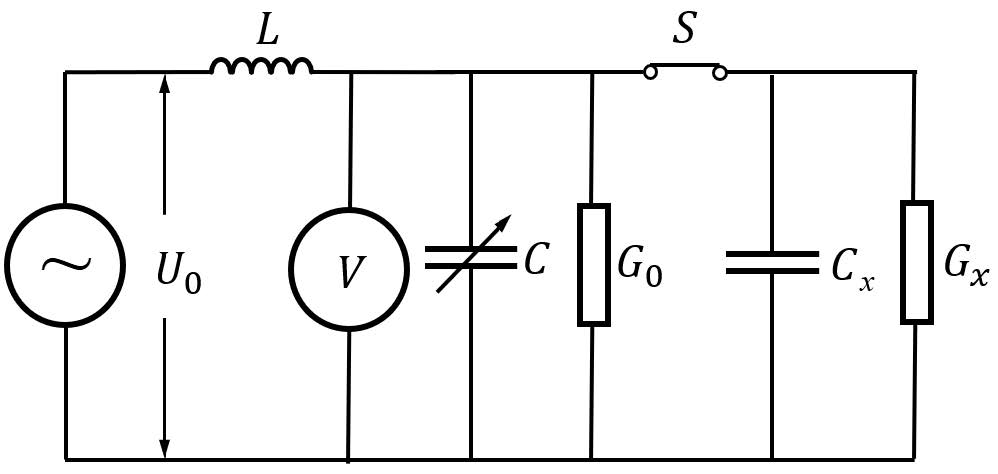
\includegraphics[width=60mm]{fg4.jpg}\
                    \caption{谐振法(Q 表法)测量电介质材料相对介电常数和介质损耗因数的原理简图\label{fig:4}}
                \end{figure}\par
            \item  WY915 测试架除了配备有平行板电容器之外,还配备了一个电容线性变化率为 \SI{0.33}{\pico\farad/\milli\metre}、长度调节范围为 0 \~{} 25 \unit{\milli\metre}、分辨率为 \SI{0.0033}{\pico\farad} 的圆筒电容器。该圆筒电容器为我们提供了另外一种测量电介质材料相对介电常数和介质损耗因数的方法(变电纳法)。
            
            1)将 Q 表调至指定频率,并接入适当电感值的标准电感和 WY915 测试架。将样品插入 WY915 测试架的平行板电容器中,并调节螺旋测微器夹紧样品,同时记录样品厚度 $D_2$。调节圆筒电容器的螺旋测微器至中央位置附近(如 12mm 处)。调节 Q 表的调谐电容使电路谐振,并读取 $Q_s$ 值(对应电压为 $U_{rs}$)。

            2)调节测试架上圆筒电容器的螺旋测微器使电路偏离谐振点(此时 Q 表充当电压表),使电压降至 $U_{rs}/\sqrt{2}$。在此电压下有两个电容值,位于最大谐振点对应的电容值 $C_r$ 两端。由此确定 $U_{rs}/\sqrt{2}$ 对应的两个电容的差值 $C_s$。

            3)调节圆筒电容器的螺旋测微器回到 12mm 处,使电路再次谐振。调节平行板电容器的螺旋测微器松开两极板,取出电介质样品,电路再次偏离谐振。调节平行板电容器的螺旋测微器改变空气隙宽度,使电路再次谐振,并读取 $Q_a$ 值(对应电压为 $U_{ra}$),同时记录空气隙的宽度 $D_4$。调节圆筒电容器的螺旋测微器使电路偏离谐振点,使电压降至 $U_{ra}/\sqrt{2}$。在此电压下有两个电容值,位于最大谐振点对应的电容值 $C_r$ 两端。由此确定与 $U_{ra}/\sqrt{2}$ 对应的两个电容的差值 $C_a$。

            4)计算所需物理量:$K$ 为圆筒电容器的线性变化率(0.33 pF/mm),$M1$ 和 $M2$ 分别为圆筒电容器螺旋测微器测得的极板间距的改变量,对应于 $\Delta C_s$ 和 $\Delta C_a$ 的电容变化量。样品厚度 $d$(cm),极板半径 $r$(cm)。

        \end{enumerate}


        \begin{figure}[!ht]\centering
            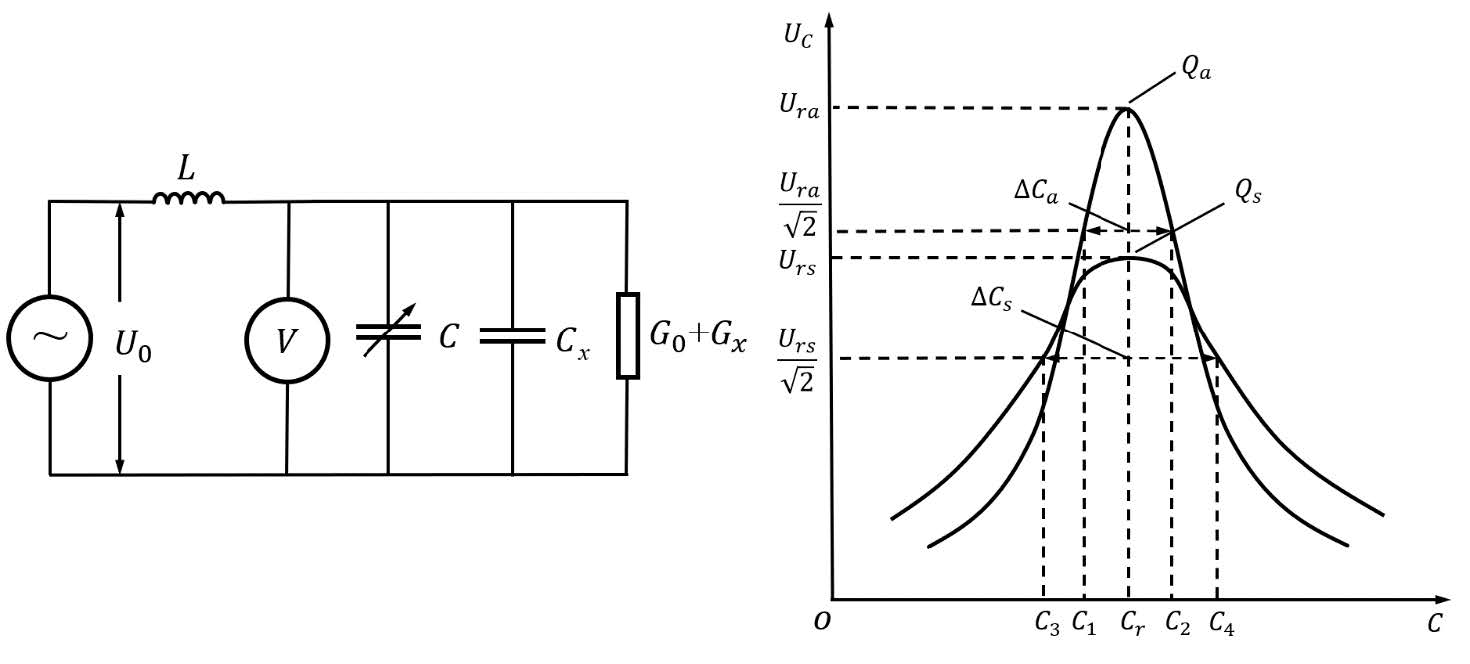
\includegraphics[width=100mm]{fg5.jpg}\
            \caption{变电纳法测量绝缘材料相对介电常数和介质损耗因数的电路图和原理图\label{fig:5}}
        \end{figure}

\newpage
\section*{【实验仪器】}%规格及参数

    WY2851 Q 表,WY915 介质损耗因数测试架,\SI{1}{\micro\henry} 标准电感,\SI{100}{\micro\henry} 标准电感,被测样品(印刷电路板、聚四氟乙烯和石英玻璃)。

\section*{【实验过程】}%简述主要过程和实验内容
①谐振法:

检查 Q 表零点并确认正常工作;检查 WY915 测试架上平行板电容器螺旋测微器的零点。

1. 将信号发生器频率调至 1 或 10 MHz 输出,并接入 100 或 1 μH 电感器至 Q 表。

2. 在平行板电容器中插入电介质样品,转动螺旋测微头至发出“吱吱”声,记录厚度 $d$。

3. 调节可变电容器使电路谐振,记录 $Q_1$ 和 $C_1$。

4. 取出电介质样品,调节圆筒电容器至 10 mm,调节 Q 表使电路谐振,记录 $Q_2$ 和 $C_2$。

5. 根据已知半径 $r^2$ 计算平行板电容器的电容 $C_p$,并根据公式计算介电常数 $\varepsilon$ 和介电损耗 $\tan\delta$。

②变电纳法:

1. 将信号发生器频率调至 1 MHz 输出,并接入 100 电感器至 Q 表。

2. 记录平行板电容器两板接触时的刻度 $D_0$,插入电介质样品并夹紧,记录 $D_1$ 并计算厚度 $D_2$。

3 调节圆筒电容器至 12 mm,调节 Q 表使电路谐振,记录 $Q_m$。

4. 调节圆筒电容器远离谐振点,记录 $1/2$ 倍 $Q_m$ 时的两端电容,计算差值 $M_1$。

5. 调节圆筒电容器至 12 mm,取出样品并调节平板电容器使电路再次谐振,记录平行板电容器间距 $D_3$ 并计算厚度 $D_4$。

6. 调节圆筒电容器远离谐振点,记录 $1/2$ 倍 $Q_m$ 时的两端电容,计算差值 $M_2$。

\section*{【实验数据】}
    表格随制作了excel表格,附后

\section*{【实验数据处理与结果分析】}

\subsection*{实验数据处理}
可计算的不确定度主要来源为螺旋测微器(精度为 $ 0.01 \unit{\milli\meter} $),可调电容读数(精度为 $0.2\unit{\pF}$)。Q表读数引入的不确定度难以确定,因此不得不忽略;平行板电极直径的测量不确定度讲义中未提及,同样忽略。假定矩形分布来评估仪器精度引入的不确定度。此处计算B类不确定度,可以得到下表:\par
Q表读数引起的不确定度不详,以及其余与仪器有关的不确定度讲义未提及,此处不做考虑。

B类不确定度:
\begin{equation*}
    u_b = k_p \cdot \Delta / C
\end{equation*}
其中,C 取$3^(1/2)$,$\Delta $取最大精度,$k_p$ 取1
\begin{table}[!ht]
    \centering\begin{tabular}{c c c}\hline
        直接测量量 & 精度 & B类不确定度 \\ \hline
        \makebox[50mm]{螺旋测微器} & $\pm 0.01 \unit{\milli\meter}$ &\makebox[50mm]{0.0057735} \\
        可调电容 & $\pm 0.2 \unit{\pF}$ & 0.11547
    \end{tabular}
\end{table}

    A类不确定度:
    \begin{equation*}
        u_a =(\frac{\Sigma (x_i-\bar{x})^2}{n(n-1)})^{1/2}
    \end{equation*}

以实验一的印刷电路板实验为例计算不确定度,计算相对介电公式为$\epsilon=\frac{3.6d (c_2-c_1)}{r^2}+1$

合成不确定度:
    $u^2={u_a}^{2} + {u_b}^{2}$

接下来,求合成标准不确定度:
    \begin{center}
        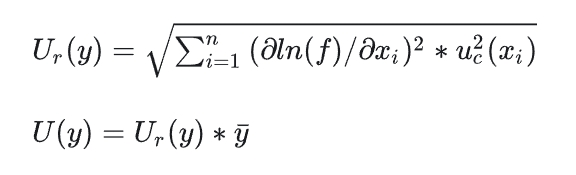
\includegraphics[width=200pt]{4.png}
    \end{center}

    $U_r^2=(\frac{\partial ln(f) }{ \partial C_1})^2 \cdot C_1^2+(\frac{\partial ln(f) }{ \partial C_2})^2 \cdot C_2^2+(\frac{\partial ln(f) }{ \partial d})^2 \cdot d^2$

其中$\frac{\partial \epsilon}{C_1} =-3.6d/r^2 $,$\frac{\partial \epsilon}{C_2} =3.6d/r^2 $,$\frac{\partial \epsilon}{d} = 3.6(C_2-C_1)/r^2$

代入得:$U_r =0.0623$

所以拓展不确定度:$\Delta N \cdot k $ = 0.0623*1.96(k=1.96)=0.122108

即:$\epsilon =6.1 \pm 0.2 \Omega \cdot cm$ 


\subsection*{结果分析}
        1.三种方法测得的相对介电常数总体上很接近,说明我们得到的数据之间有相互印证的关系,数据的
        可靠性比较高,同时因为不同的样品之间的介电常数等值会因为填料等成分差距而有不同,所以难以找到参考值。

        2.印刷电路板:三种方法测得的相对介电常数相对接近,但是偏差在10\%左右,同时,介质损耗因数也有一定差距。

        3.聚四氟乙烯:三种方法测得的相对介电常数相对接近,但是10Mhz下测得的相对介电常数有明显的降低,可能在操作过程中有一定失误。

        4.石英玻璃:三种方法测得的相对介电常数相对接近,一定程度上也表面实验情况还可以。

        5.可以改进的点:在实验中要特别注意空气隙对测量结果的影响,确保测量时能够达到螺旋测微器最小刻度值的精度。

        对于样品的处理,可以采取一些方法来保证其表面整洁和平整,例如戴手套用镊子夹取样品,以确保样品与测量设备无缝接触。
        
        温度和湿度是影响测量结果的重要环境因素,应该对其进行控制或者考虑温度修正系数来修正结果。
        
        在实验中要注意使用稳定的标准设备,避免接触不良或者受到周围环境的扰动,以确保准确的测量结果。
    



\section*{【思考题】}

\begin{center}
    一、介质损耗的根源是什么?
\end{center}
介质损耗是指电介质材料在外电场作用下因发热而引起的功率损耗。
电介质在受到外电场作用时会产生发热现象,表明部分电能已经被转化为热能并散失掉。介质损耗指的是在电介质受到电场作用下,在单位时间内因发热而消耗的能量,通常称为电介质的损耗功率,或简称介质损耗。介质损耗是衡量电介质在交流电场中性能的重要品质指标之一。它不仅导致电能的浪费,还会使元件发热,影响其正常工作。如果介电损耗过大,甚至可能引起介质的过热而导致绝缘破坏。
\begin{center}
    二、影响测量结果准确性的因素有哪些?应如何做才能保证测试结果的精度?
\end{center}
\begin{enumerate}
    \item 人为确定Q表谐振状态不够准确,对于读书有一定影响。想要准确读数,可以选用更好的方法,让
    计算机记录Q表的值来确定何时谐振,或者可以小心地调整,也可以使结果更准确。
    \item 环境温度和湿度对相对介电常数和介质损耗因数测试结果有较大的影响。可以对于具体的温度和湿度对结果进行修正。
    \item 灰尘等的环境污染,样品上的灰尘和油污也会影响测试结果,可以先用酒精
    清洗再测试,测试时戴手套、用镊子夹持。
    \item 电容、极板、样品与设备的接触情况,若这些部件安装情况不良,则会影响示数,需要安装的时候提前固定好,并减少对他们的触碰。
    \item 实验仪器精度问题。更换更好的仪器,或者使用误差更小的方法进行测量。
\end{enumerate}


\end{document}